\setAuthor{Konstantin Dukatš}
\setRound{lahtine}
\setYear{2021}
\setNumber{G 3}
\setDifficulty{3}
\setTopic{TODO}

\prob{Kumerpeegel}
Joonisel on kujutatud kumerlääts, selle optiline peatelg ning üks fookustest. On teada, et kusagil optilises skeemis leidub ka kumerpeegel. Kui panna valgusallikas punktidesse $S_1$ või $S_2$, siis tekkinud kujutis kattub allikaga. Konstrueerige kumerpeegel. Esitage lahendus lisalehel.
\begin{figure}[h]
  \vspace{-1em}
  \centering
  \resizebox{\textwidth}{!}{%
  \begin{tikzpicture}[scale=1]
    \filldraw[black] (2,0) circle (1.5pt) node[anchor=south] {$F$};
    \filldraw[black] (0,0) circle (1.5pt) node[anchor=south west] {$O$};
    \filldraw[black] (-3.6,0) circle (1.5pt) node[anchor=south] {$S_2$};
    \filldraw[black] (-6,0) circle (1.5pt) node[anchor=south] {$S_1$};


    \draw[gray] [dashed,-] (-7,0) -- (7,0);
    \draw[line width=1pt,Stealth-Stealth] (0,-2) -- (0,2);
  \end{tikzpicture}
  }%
  \vspace{-1em}
\end{figure}



\hint

\solu
Konstrueerime esmalt punktide $S_1$ ja $S_2$ kujutised $S_1'$ ja $S_2'$".
\begin{figure}[h]
  \centering
  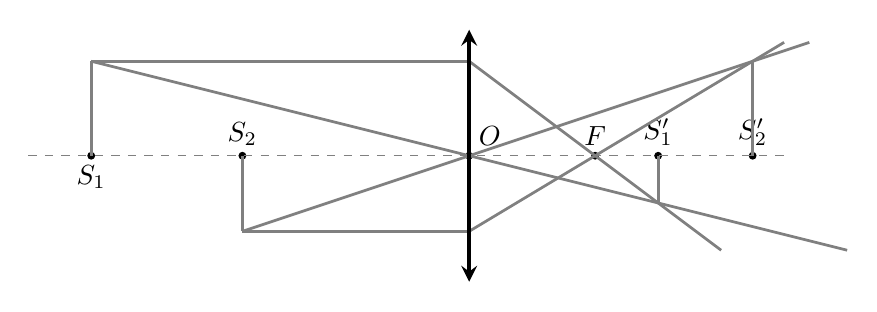
\begin{tikzpicture}[scale=0.8]
    \filldraw[black] (2,0) circle (1.5pt) node[anchor=south] {$F$};
    \filldraw[black] (0,0) circle (1.5pt) node[anchor=south west] {$O$};
    \filldraw[black] (-3.6,0) circle (1.5pt) node[anchor=south] {$S_2$};
    \filldraw[black] (-6,0) circle (1.5pt) node[anchor=north] {$S_1$};

    \filldraw[black] (4.5,0) circle (1.5pt) node[anchor=south] {$S^\prime_2$};
    \filldraw[black] (3,0) circle (1.5pt) node[anchor=south] {$S^\prime_1$};

    \draw[gray] [dashed,-] (-7,0) -- (5,0);
    \draw[gray, line width=1pt] (-6,0) -- (-6,1.5);
    \draw[gray, line width=1pt] (-6,1.5) -- (6,-1.5);
    \draw[gray, line width=1pt] (3,-0.75) -- (3,0);
    \draw[gray, line width=1pt] (-6,1.5) -- (0,1.5);
    \draw[gray, line width=1pt] (0,1.5) -- (4,-1.5);

    \draw[gray, line width=1pt] (-3.6,0) -- (-3.6,-1.2);
    \draw[gray, line width=1pt] (-3.6,-1.2) -- (5.4,1.8);
    \draw[gray, line width=1pt] (4.5,1.5) -- (4.5,0);
    \draw[gray, line width=1pt] (-3.6,-1.2) -- (0,-1.2);
    \draw[gray, line width=1pt] (0,-1.2) -- (5,1.8);

    \draw[line width=1.5pt,>=stealth, <->] (0,-2) -- (0,2);
  \end{tikzpicture}
\end{figure}

Teame, et kui valguskiir langeb peegelpinnale risti, siis liigub see samasugust teed pidi tagasi alguspunkti suunas. Tänu kiirte pööratavuse printsiibile jõuab valguskiir punktidest $S_1'$ ja $S_2'$ tagasi vastavatesse algpunktidesse $S_1$ ja $S_2$. Kumerpeegel on sfääriline, seejuures punkti $S_2'$ poole suunatud kiirte pikendused määravad ära peegli keskpunkti ning punktide $S_1'$ ja $S_2'$ vahekaugus määrab ära joonistatava kaare raadiuse.

\begin{figure}[h]
  \centering
  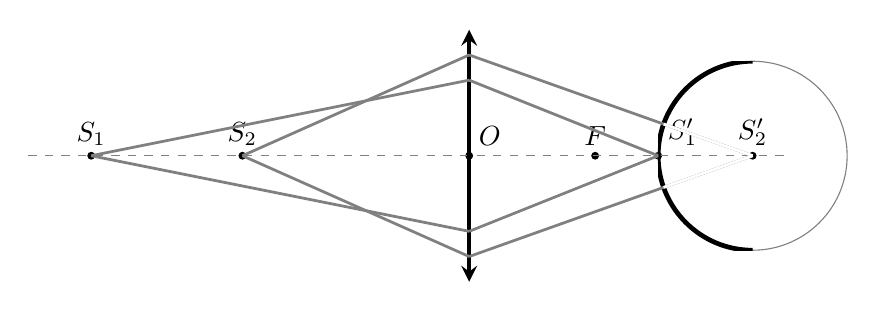
\begin{tikzpicture}[scale=0.8]
    \filldraw[black] (2,0) circle (1.5pt) node[anchor=south] {$F$};
    \filldraw[black] (0,0) circle (1.5pt) node[anchor=south west] {$O$};
    \filldraw[black] (-3.6,0) circle (1.5pt) node[anchor=south] {$S_2$};
    \filldraw[black] (-6,0) circle (1.5pt) node[anchor=south] {$S_1$};

    \filldraw[black] (4.5,0) circle (1.5pt) node[anchor=south] {$S^\prime_2$};
    \filldraw[black] (3,0) circle (1.5pt) node[anchor=south west] {$S^\prime_1$};

    \draw[gray] [dashed,-] (-7,0) -- (5,0);
    \draw[gray] (4.5,0) circle (1.5);
    \draw[line width=1.5pt,>=stealth, <->] (0,-2) -- (0,2);

    \begin{scope}
      \clip (3,-1.5) rectangle (4.5,1.5);
      \draw[black, line width=1.7pt] (4.5,0) circle(1.5);
    \end{scope}

    \draw[gray, line width=1pt] (-6,0) -- (0,-1.2);
    \draw[gray, line width=1pt] (0,-1.2) -- (3,0);
    \draw[gray, line width=1pt] (-6,0) -- (0,1.2);
    \draw[gray, line width=1pt] (0,1.2) -- (3,0);

    \draw[gray, line width=1pt] (-3.6,0) -- (0,-1.6);
    \draw[gray, line width=1pt] (0,-1.6) -- (4.5,0);
    \draw[gray, line width=1pt] (-3.6,0) -- (0,1.6);
    \draw[gray, line width=1pt] (0,1.6) -- (4.5,0);
    \begin{scope}
      \clip (3,-1.5) (4.5,0) circle(1.5);
      \draw[white, line width=1pt] (0,1.6) -- (4.5,0);
      \draw[white, line width=1pt] (0,-1.6) -- (4.5,0);
    \end{scope}

  \end{tikzpicture}
\end{figure}
\probend